\documentclass[../main.tex]{memoir}

\begin{document}

\chapter{Estado del arte en análisis de multitudes en
  videovigilancia}
\label{sec:state-of-the-art}

En este capítulo se va a realizar un análisis sobre el estado del arte
en el análisis de comportamientos en videovigilancia. El contenido de
este capítulo consiste en un resumen de las ideas fundamentales que
aparecen en el artículo ``Revisiting crowd behaviour analysis through
deep learning: Taxonomy, anomaly detection, crowd emotions, datasets,
opportunities and prospects''. Este artículo se ha redactado tras una
investigación durante este curso académico, y está aceptado para
publicación en la revista \textit{Information Fusion}.

\section{Propuesta taxonómica}

En esta sección se introduce una propuesta taxonómica para la
organización de los trabajos que abordan el análisis de
comportamientos en multitudes. Esta taxonomía aparece tras el análisis
de las propuestas anteriores, en las que se observa una carencia de
estructura que organice las distintas tareas que componen el área.

\subsection{Categorizaciones previas}

La categorización más utilizada para la organización de los trabajos
que se engloban dentro de esta área es la propuesta en
\cite{zitouni2016advances}. Dicha estructuración divide los trabajos
que se engloban dentro del análisis de comportamientos en multitudes
en cuatro subproblemas:

\begin{itemize}
\item Clasificación de comportamientos: Esta tarea consiste en
  identificar y clasificar los comportamientos presentes en el vídeo
  dentro de un conjunto de comportamientos conocidos de antemano.
\item Conteo de individuos: Esta tarea consiste en estimar el número
  de individuos presentes en cada fotograma.
\item Detección y seguimiento de individuos: En esta tarea se engloban
  los trabajos cuyo objetivo es el seguimiento de la trayectoria de
  los individuos en el vídeo.
\item Detección de comportamientos anómalos: En este caso, se trata de
  identificar cuándo se produce un comportamiento anormal o
  desconocido en la secuencia de vídeo.
\end{itemize}

Dicha taxonomía ha sido utilizada como referencia a la hora de
realizar estudios posteriores del estado del arte en la temática
\cite{swathi2017crowd}. Esta categorización incluye las tareas
principales dentro de este ámbito de estudio, pero sitúa todas las
tareas al mismo nivel. No obstante, existe claramente una organización
jerárquica entre las tareas listadas, y pueden organizarse las mismas
siguiendo una secuencia. Por ejemplo, el conteo de individuos suele
venir precedido por una etapa de detección de individuos en la escena.
Además, la salida del conteo puede utilizarse en etapas posteriores
para detectar situaciones anómalas, como una excesiva congestión en
una aglomeración de personas. La taxonomía que se propone establece
una jerarquía entre las diferentes tareas, al tiempo que mantiene las
aportaciones de los trabajos anteriores como etapas dentro de la
jerarquía.

\subsection{Taxonomía propuesta}

Con la taxonomía propuesta a continuación se pretende establecer una
conexión entre las distintas subtareas que aparecen dentro de esta
área de conocimiento. La propuesta se vertebra en torno a dos
ejes complementarios:

\begin{itemize}
\item Por un lado, hay dos formas principales de afrontar el análisis
  de comportamientos en multitudes, en función de la relación que se
  establece entre los individuos aislados y la multitud que
  forman. Esta distinción se traduce en los enfoques microscópico y
  macroscópico, que se explicarán más adelante.
\item Por otro lado, independientemente del enfoque seleccionado, las
  diferentes tareas se organizan en cuatro etapas. Usualmente, las
  etapas posteriores suelen tener una fuerte dependencia en las etapas
  previas.
\end{itemize}

En la figura \ref{fig:pipeline} puede apreciarse visualmente la
organización anterior en dos ejes. Dicha organización muestra la
interdependencia entre las dos organizaciones anteriores. Todas las
etapas de la jerarquía pueden llevarse a cabo utilizando cualquiera de
los dos enfoques. No obstante, la elección del enfoque microscópico o
macroscópico producirá ligeras diferencias en la solución obtenida.

\begin{figure}[hbtp]
  \centering
  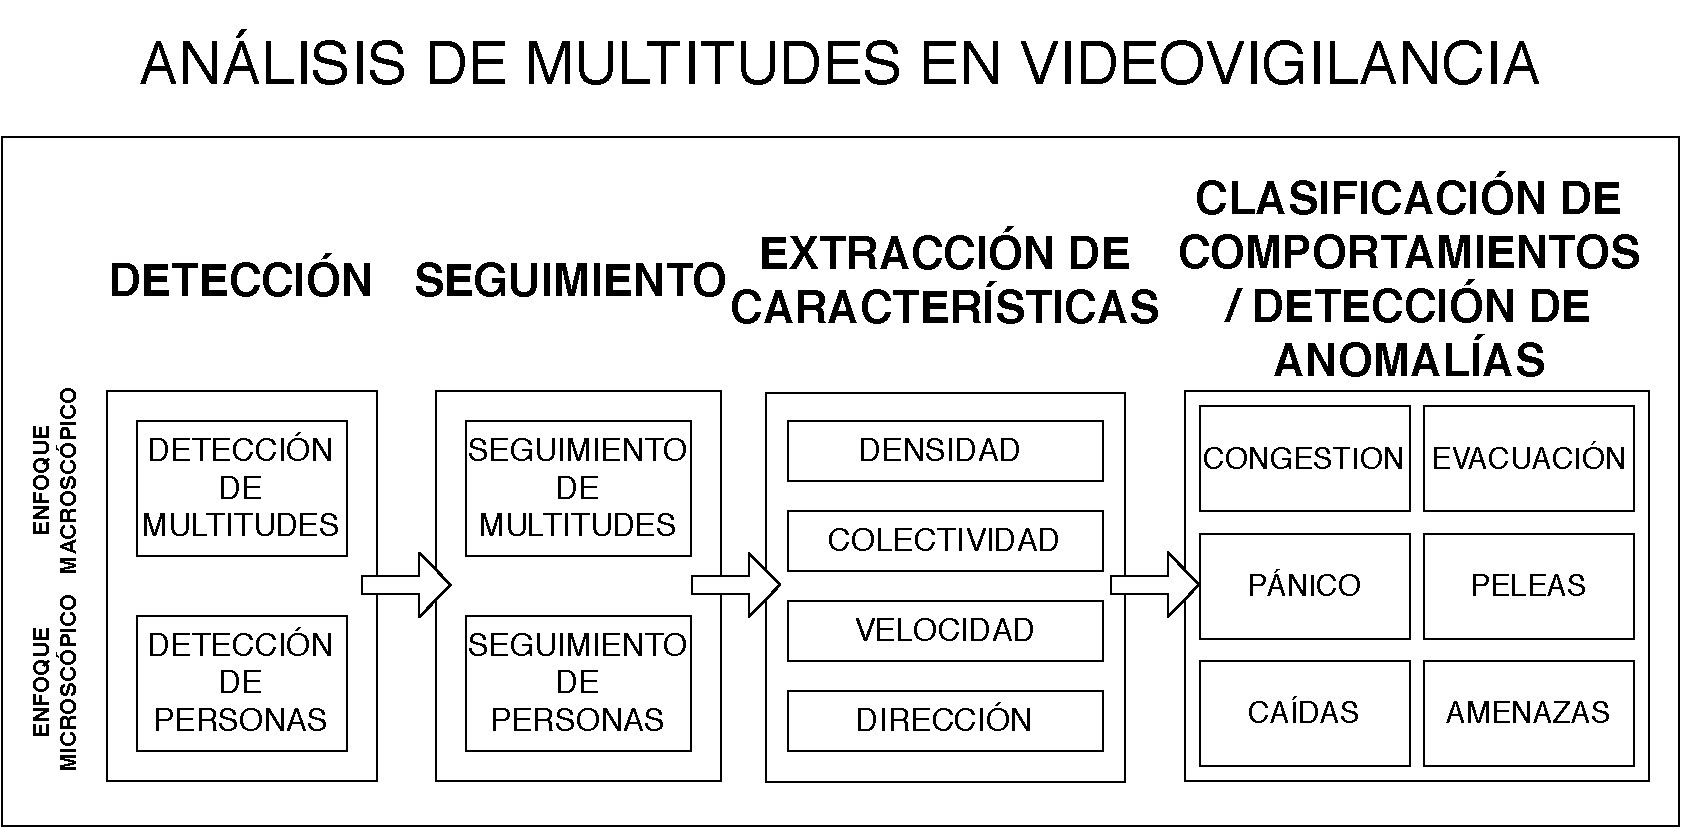
\includegraphics[width=.9\textwidth]{images/taxonomy_steps.pdf}
  \caption{Propuesta taxonómica. En ella puede verse la organización
    de los trabajos en cuatro etapas consecutivas}
  \label{fig:pipeline}
\end{figure}

\subsubsection{Enfoque macroscópico contra enfoque microscópico}

La primera distinción distribuye los trabajos en función de cómo se
consideran los individuos en relación con la multitud a la que
pertenecen. Como hemos dicho anteriormente, esta categorización no
forma parte de la jerarquía, sino que es una clasificación
complementaria que influye en gran medida a las distintas etapas. Los
dos enfoques principales son los que siguen:

\begin{itemize}
\item Enfoque microscópico: En este caso, se trata a la multitud como
  una colección de individuos. Las distintas personas que aparecen en
  el vídeo se estudian individualmente, y posteriormente se relaciona
  la información obtenida de las mismas para inferir la información a
  nivel de multitud.
\item Enfoque macroscópico: Estos son enfoques holísticos, en los que
  la multitud es tratada como un ente único y completo, sin necesidad
  de estudiar individualmente a las personas que la componen.
\end{itemize}

Normalmente, los enfoques microscópicos tienden a arrojar mejores
resultados cuando los individuos pueden ser estudiados de forma
aislada correctamente. Esto es, en entornos en los que los individuos
son claramente visibles, las oclusiones son pequeñas, y la densidad de
personas es baja. Por otra parte, cuando la densidad de individuos
aumenta, la calidad de los algoritmos de seguimiento se degrada
significativamente. En estas circunstancias, los enfoques
macroscópicos suelen ser más adecuados, ya que los individuos
específicos dejan de ser el objetivo, y se pasa a estudiar la multitud
de forma completa.

\subsubsection{Jerarquía de tareas}
\label{sec:crowd-analysis-pipeline}

Independientemente del enfoque escogido, la jerarquía de tareas
incluye las cuatro fases indicadas en la figura \ref{fig:pipeline}:

\begin{enumerate}
\item Detección: El objetivo de esta fase es localizar la posición de
  los individuos (en los enfoques microscópicos) o las multitudes (en
  los macroscópicos) en cada fotograma. Esta etapa ha sido ampliamente
  estudiada con anterioridad, y existen diversos modelos con gran
  precisión y rendimiento \cite{nguyen2016human}
\item Seguimiento de individuos: Se trata de identificar unívocamente
  a las personas o multitudes durante una secuencia de fotogramas
  consecutivos. En el caso de multitudes, se suelen calcular también
  los flujos de movimiento dominantes \cite{garate2009crowd}. De nuevo,
  es un área ampliamente estudiada \cite{ciaparrone2020deep}.
\item Extracción de características: El objetivo de esta etapa
  consiste en el cómputo de una serie de métricas que describan la
  dinámica de la multitud o los individuos en escena. Algunos ejemplos
  de estas características pueden ser la velocidad o dirección de las
  trayectorias, o la densidad de individuos.
\item Clasificación de comportamientos y detección de anomalías:
  Utilizando como base las características extraídas en la etapa
  anterior, este paso trata de reconocer comportamientos particulares
  o situaciones anómalas en la secuencia de vídeo. En función del
  paradigma de aprendizaje utilizado, existen dos posibles enfoques
  para esta etapa:
  \begin{itemize}
  \item La clasificación de comportamientos engloba a los trabajos que
    utilizan un enfoque supervisado, los cuales tratan de asignar una
    clase conocida previamente al comportamiento a clasificar.
  \item La detección de anomalías trata de identificar patrones anómalos
    utilizando un enfoque no supervisado para resolver el problema.
  \end{itemize}
\end{enumerate}

Las dos últimas etapas de la jerarquía van a ser analizadas en mayor
profundidad en las secciones posteriores. Las dos primeras secciones
han sido ampliamente estudiadas con anterioridad, por lo que
excluiremos su análisis en este trabajo.

\subsubsection{Características relevantes para el estudio de multitudes}

Tras las etapas de detección y seguimiento de individuos o multitudes
en la escena, suele encontrarse una etapa de extracción de
características. A pesar de que la información extraída puede ser de
muy diversa índole, se han identificado como relevantes las siguientes
características, debido a que un amplio número de trabajos utilizan
alguna de ellas en su funcionamiento. Dichas características son:

\begin{itemize}
\item Velocidad: Mide la velocidad media a la que se mueven los
  individuos o la multitud en la escena.
\item Dirección: En el enfoque macroscópico, número de direcciones
  principales de movimiento presentes en la multitud. En el
  microscópico, se puede extraer la dirección de cada uno de los
  individuos en escena.
\item Densidad o conteo: Mide el número de individuos presentes
  en la imagen, o la proximidad que existe entre ellos cuando se
  estudian multitudes completas.
\item Colectividad o cohesión: Esta característica mide la fuerza con
  la que se relacionan los individuos que conforman la multitud.
  Cuando una persona forma parte de un grupo grande, en lugar de
  comportarse individualmente, tiende a imitar el comportamiento de
  los individuos que le rodean, asimilando su dirección y velocidad.
  De esta forma, aparecen estructuras coherentes debidas al
  movimiento. La colectividad trata de medir la estabilidad de dichas
  estructuras, y depende de múltiples factores.
\end{itemize}

Adicionalmente, la etapa de extracción de características puede
llevarse a cabo con un modelo de aprendizaje profundo, que aprenda a
seleccionar las características más relevantes para la tarea que se
trata de resolver. Este enfoque en particular es el que utilizaremos
en la experimentación práctica del trabajo, donde un modelo
espacio-temporal será el encargado de aprender las características
relevantes.

\subsubsection{Clasificación de comportamientos y detección de anomalías}
\label{sec:behavior-classification-and-anomaly}

Las características extraídas en la etapa anterior tienen que ser
resumidas para obtener información relevante sobre la multitud
estudiada. Como hemos explicado anteriormente, existen dos enfoques
principales para abordar esta etapa. Por un lado, tenemos la
clasificación de comportamientos, en la que los modelos se entrenan
utilizando un paradigma supervisado sobre las características
extraídas, y la detección de anomalías, en la que el aprendizaje se
realiza desde el punto de vista no supervisado. La monitorización de
las características a lo largo del tiempo permite la detección de
comportamientos anómalos en la multitud, especialmente cuando se
producen cambios bruscos en dichas métricas. Por ejemplo, un aumento
repentino de la velocidad media de los individuos en la imagen puede
ser un indicador de alerta, ya que puede estar ocurriendo una
estampida, o una congestión puede ser expresada en términos de
alta densidad y baja velocidad.\\

Cuando el problema se resuelve desde el punto de vista de la detección
de anomalías, otra posible clasificación aparece en función de la
fuente que produce la anomalía. El motivo por el que ocurre el evento
anómalo puede ser de diversa índole, y por lo tanto la forma de afrontar
el problema puede ser ligeramente distinta. Se han identificado cuatro
principales fuentes de anomalía en la revisión de la literatura:

\begin{itemize}
\item Posición anómala: Esta anomalía ocurre cuando un objeto tiene
  una posición atípica en la escena. Ocurre normalmente cuando un
  individuo se en una zona no autorizada, por ejemplo. Es la anomalía
  más simple de las estudiadas, ya que usualmente se resuelve con una
  fase de detección de personas y cálculo de solapamiento entre la
  detección y la zona restringida.
\item Movimiento anómalo: En este caso, la anomalía ocurre porque se
  detecta una trayectoria inesperada, bien por un único individuo o por
  un grupo. Hay dos posibles fuentes de irregularidad en este caso: la
  velocidad, cuando alguien se mueve más rápido o más lento que la
  gente que lo rodea, y la dirección, cuando hay flujos de movimiento
  predominantes y una trayectoria se desvía significativamente de los
  mismos.
\item Apariencia anómala: Esta anomalía se produce cuando un objeto no
  identificado aparece en la escena. Un ejemplo típico de esta anomalía
  es la presencia de vehículos en zonas peatonales.
\item Acción anómala: Es la anomalía más difícil de detectar dentro de
  las comentadas. Conlleva el aprendizaje de los patrones de
  comportamiento habituales para una escena determinada, y la detección
  de patrones poco comunes.
\end{itemize}

En la práctica, muchas de estas anomalías aparecen combinadas. Por
ejemplo, es típico que la anomalía de movimiento y la de apariencia
aparezcan simultáneamente en los conjuntos de datos. En particular, en
el UCSD Pedestrian Dataset \cite{mahadevan2010anomaly}, el más
utilizado en la temática, aparecen tanto ejemplos de movimiento
anómalo como vehículos no autorizados en una calzada peatonal. Pueden
observarse distintos ejemplos de anomalía presentes en conjuntos de
datos públicos en la figura \ref{fig:anomalies}.

\begin{figure}[hbtp]
  \centering
  \begin{subfigure}{0.48\textwidth}
    \centering
    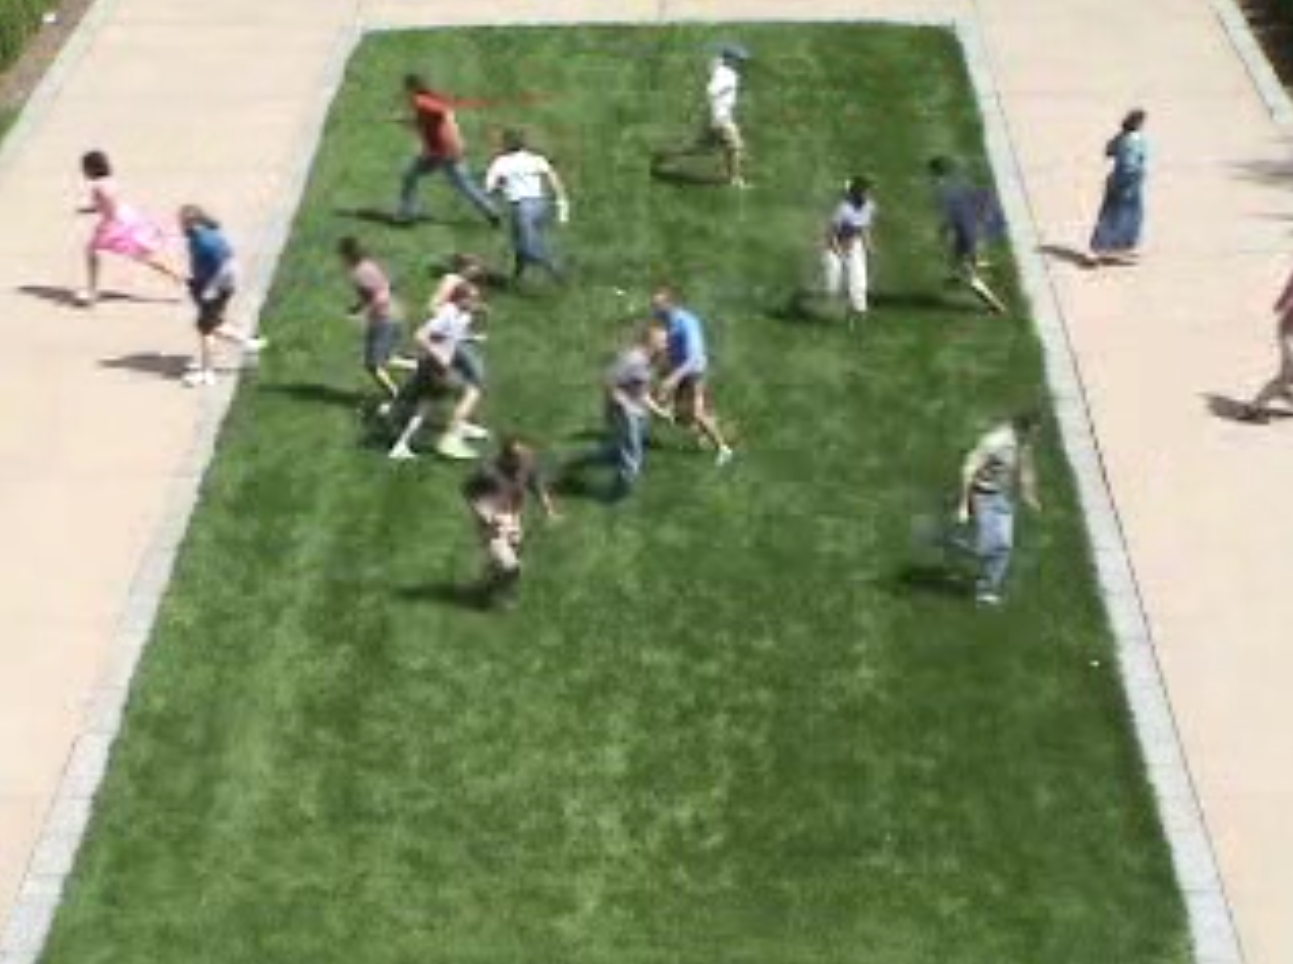
\includegraphics[width=.9\linewidth]{images/umn-anomaly}
    \caption{Ejemplo de anomalía en el UMN Dataset
      \cite{mehran2009abnormal}. En el vídeo, una multitud poco
      estructurada se desplaza por la imagen. En cierto momento, el
      movimiento pasa a ser acelerado por una situación de pánico, así
      que se produce una anomalía de movimiento}
  \end{subfigure}
  \begin{subfigure}{0.48\textwidth}
    \centering
    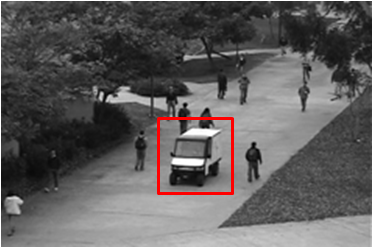
\includegraphics[width=.9\linewidth]{images/ucsd-anomaly}
    \caption{Ejemplo de anomalía en el UCSD Pedestrian Dataset
      \cite{mahadevan2010anomaly}. Dado que no se permite la
      circulación de vehículos por esa acera, la presencia del coche
      es una anomalía de apariencia.}
  \end{subfigure}
  \begin{subfigure}{0.48\textwidth}
    \centering
    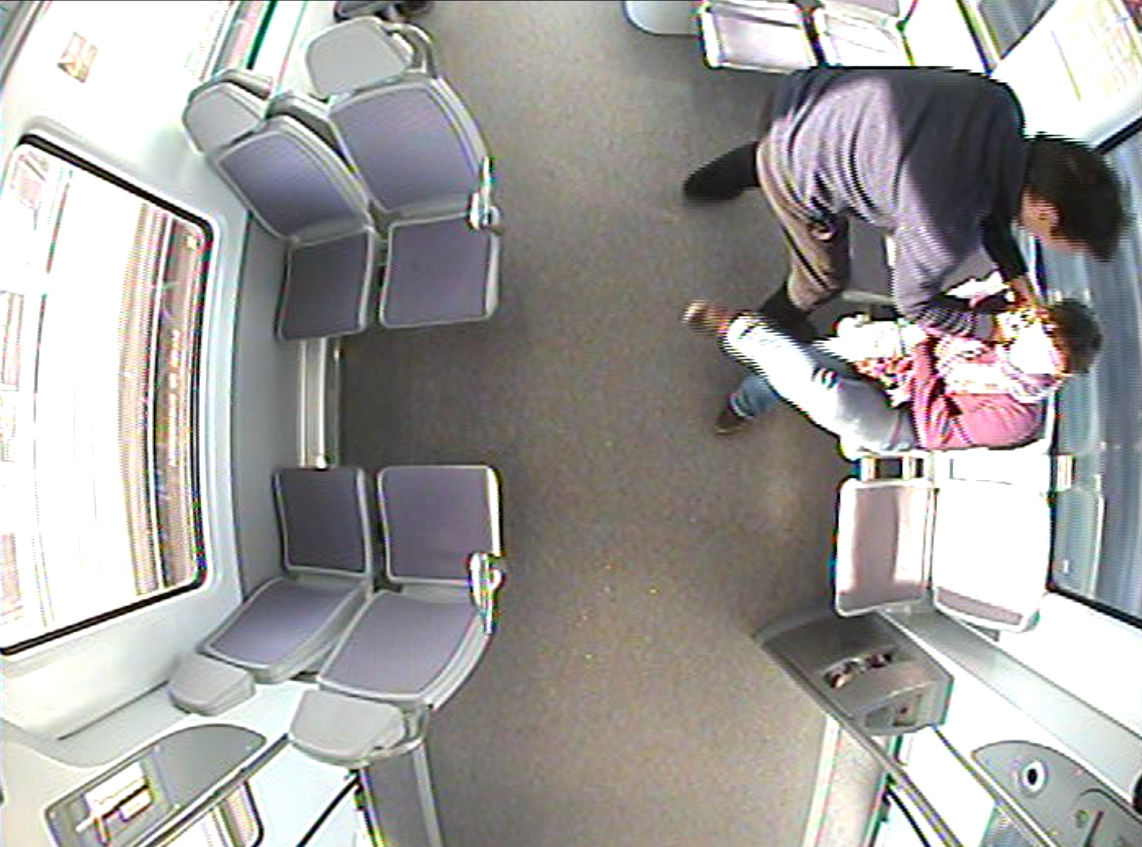
\includegraphics[width=.9\linewidth]{images/boss-anomaly}
    \caption{Ejemplo de acción anómala en el BOSS Dataset
      \cite{velastin2017people}. En este caso, el hombre roba el
      teléfono a la mujer mientras está hablando.}
  \end{subfigure}
  \begin{subfigure}{0.48\textwidth}
    \centering
    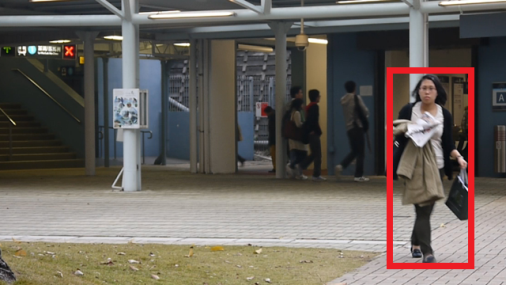
\includegraphics[width=.9\linewidth]{images/avenue-anomaly}
    \caption{Ejemplo de anomalía de movimiento en el conjunto de datos
      CUHK Avenue Dataset \cite{lu2013abnormal}. En este conjunto de
      datos, el plano de movimiento normal es paralelo al plano de la
      cámara, por lo que un movimiento en dirección perpendicular se
      considera un patrón anómalo de movimiento.}
  \end{subfigure}
  \caption{Ejemplos de anomalías en los distintos conjuntos de datos.}
  \label{fig:anomalies}
\end{figure}


\section{Conjuntos de datos públicos para detección de anomalías en multitudes}

Debido a la diversidad que existe en la tarea de detección de
comportamientos anómalos en multitudes, existe una gran cantidad de
conjuntos de datos distintos disponibles públicamente. Cada conjunto
de datos se centra en una o varias de las categorías de anomalía que
hemos listado anteriormente. En esta sección se detallarán los
principales conjuntos de datos en función de la anomalía que
presenten. En la tabla \ref{tab:datasets} se resumen las principales
características de todos los conjuntos de datos que se han estudiado.

{\footnotesize
\ctable[ caption={Conjuntos de datos para detección de anomalías en multitudes.}, doinside=\hspace*{-2cm}, label={tab:datasets}]{lcccccc}{
    \tnote[a]{Sólo uno de los vídeos está etiquetado.}
    \tnote[b]{La etiquetación permite también la clasificación de comportamientos.}
    \tnote[c]{Vídeos normales junto con 13 clases de comportamientos anómalos.}
    \tnote[d]{Vídeos de corta duración divididos en violencia y no violencia.}
}{
    \toprule
    \multirow{2}{*}{Conjunto de datos} & \multicolumn{3}{c}{Nº fotogramas} & \multirow{2}{*}{\makecell{Nº eventos\\anómalos}} & \multirow{2}{*}{\makecell{Tipo de\\anomalía}} & \multirow{2}{*}{\makecell{Descripción de\\las anomalías}} \\ \cmidrule{2-4}
                             &  Total & Entrenamiento & Test & & & \\
    \toprule
    UCSD Peds 1 & 14000 & 6800 & 7200 & 40 & \makecell{Movimiento +\\apariencia} & \makecell{Direcciones extrañas,\\velocidad, vehículos\\no autorizados} \\
    \midrule
    UCSD Peds 2 & 4560 & 2550 & 2010 & 12  & \makecell{Movimiento +\\apariencia} &  \makecell{Direcciones extrañas,\\velocidad, vehículos\\no autorizados} \\
    \midrule
    CUHK Avenue & 30652 & 15328 & 15324 & 47  & \makecell{Movimiento +\\apariencia} & \makecell{Direcciones extrañas,\\velocidad, vehículos\\no autorizados} \\
    \midrule
    \makecell[l]{ShangaiTech\\Campus} & 317398 & 274515 & 42883 & 130 & \makecell{Movimiento +\\apariencia} & \makecell{Direcciones y velocidades\\anómalas, merodeo} \\
    \midrule
    UMN Dataset & 7725 & - & - & 3 & Movimiento & \makecell{Multitud despavorida\\instantáneamente} \\
    \midrule
    \makecell[l]{BEHAVE\\Interactions} & 225019 & - & - & 14\tmark[a] & Acción & Peleas, persecuciones \\
    \midrule
    CAVIAR & 26402 & - & - & 11\tmark[b] & Acción & \makecell{Objetos abandonados,\\peleas, caídas} \\
    \midrule
    BOSS & 48624 & - & - & 10 & Acción & \makecell{Peleas, robos,\\caídas} \\
    \midrule
    UT Interactions & 41373 & - & - & 48 & Acción & \makecell{Puñetazos,\\patadas,\\empujones} \\
    \midrule
    UCF Crime & 13M & - & - & - & Acción & \makecell{Comportamientos\\peligrosos\tmark[c]} \\
    \midrule
    Peliculas & 4991 & - & - & 100\tmark[d] & Acción & Violencia \\
    \midrule
    Hockey Fights & 41056 & - & - & 500\tmark[d] & Acción & Violencia \\
    \bottomrule
}
}

\subsection{Conjuntos de datos para la detección de movimientos anómalos}
\label{sec:motion-anomaly-datasets}

Los conjuntos de datos listados en esta sección están diseñados para
presentar patrones anómalos de movimiento. Estas anomalías están
definidas normalmente por velocidades o direcciones que se desvían de
los flujos de movimiento normales de la escena. Además, la presencia
de elementos no autorizados es común en estos conjuntos, como
vehículos o bicicletas en zonas de tránsito de peatones. Esto hace que
normalmente se considere simultáneamente el problema de detección de
movimientos y apariencias anómalas. Los conjuntos de datos más utilizados
en este contexto son los siguientes:

\begin{description}
\item[UCSD Pedestrian Dataset] Los conjuntos \textit{UCSD anomaly
    detection datasets}\footnote{UCSD dataset disponible en:
    \url{http://www.svcl.ucsd.edu/projects/anomaly/dataset.htm}}
  \cite{mahadevan2010anomaly} son los conjuntos de datos más populares
  en la literatura. Hay dos conjuntos de datos diferentes, llamados
  Peds1 y Peds2. Peds1 contiene 34 vídeos de entrenamiento y 36 de
  test y Peds2, 16 de entrenamiento y 12 de test. Cada vídeo dura
  aproximadamente 200 fotogramas (20 segundos), y están grabados a una
  resolución de 158x238 píxeles. La principal diferencia entre los dos
  conjuntos es la dirección en la que se mueven los peatones. En
  Peds1, la gente se mueve en dirección perpendicular al plano de la
  cámara, mientras que en Peds2 la dirección predominante es paralela.
  En los conjuntos de datos de entrenamiento no aparecen trayectorias
  anómalas, con el fin de mostrar los patrones de movimiento que se
  consideran usuales. En el conjunto de test, un fotograma se
  considera anómalo si hay algún elemento extraño en la imagen
  (bicicletas, monopatines, etc), o si un viandante presenta un patrón
  extraño de movimiento (velocidad anormalmente alta, o dirección no
  predominante. En total, unos 3400 fotogramas son anómalos, frente a
  unos 5500 que son normales.  Hay dos formas distintas de marcar las
  anomalías:
  \begin{itemize}
  \item Para cada vídeo hay una marca binaria por fotograma, indicando
    si el mismo es anómalo o no (anotaciones a nivel de fotograma)
  \item Adicionalmente, para 10 vídeos de Peds1, se adjuntan máscaras
    que indican la posición exacta de la anomalía dentro del fotograma
    (anotaciones a nivel de píxel).
  \end{itemize}
  A pesar de ser el conjunto de datos más empleado en la literatura,
  resulta difícil comparar los trabajos que lo utilizan, debido a que
  no existe una tabla de resultados centralizada. La mayoría de
  trabajos que utilizan este dataset resuelven simultáneamente la
  detección de movimientos y apariencias anómalas, dado que en las
  anotaciones del conjunto de datos no se hace distinción en la fuente
  de la anomalía.
\item[CUHK Avenue Dataset] El conjunto de datos CUHK
  Avenue\footnote{El conjunto CUHK Avenue se puede descargar de
    \url{http://www.cse.cuhk.edu.hk/leojia/
      projects/detectabnormal/dataset.html}} \cite{lu2013abnormal}
  está compuesto por 16 vídeos de entrenamiento (15328 fotogramas) y
  21 de test (15324 fotogramas). De nuevo, se consideran trayectorias
  normales aquellas que se mueven en un plano paralelo a la cámara,
  mientras que la gente moviéndose en otras direcciones, con patrones
  de movimiento extraños o los vehículos se consideran anomalías. En
  este caso, las anotaciones marcan las anomalías con un rectángulo, y
  el criterio de evaluación es la métrica IoU (\textit{intersection
    over union}, se explicará más adelante) entre la detección y la
  anotación.
\item[UMN dataset] El conjunto de datos UMN\footnote{UMN está
    disponible en \url{http://mha.cs.umn.edu/proj\_events.shtml\#crowd}}
  es un conjunto de datos sintético compuesto por tres escenas, con
  una longitud total ligeramente superior a los 4 minutos (7725
  fotogramas). En cada uno de los vídeos se muestra una multitud poco
  cohesiva, que repentinamente empieza a correr en todas direcciones.
  El momento en el que se produce el cambio de velocidad se considera
  como inicio de la anomalía. Esta tarea puede verse alternativamente
  como detección de movimiento anómalo o como detección de acción
  anómala. Esto se debe a que la anomalía está producida por un cambio
  brusco de velocidad y dirección, características fuertemente
  relacionadas con las anomalías de movimiento, pero los patrones de
  movimiento en la escena están completamente desestructurados, en
  contraste con el movimiento estructurado de los conjuntos previos.
  Esta falta de estructura hace que no sea posible aprender los
  principales flujos de movimiento, por lo que las aproximaciones
  usuales al problema del movimiento anómalo son difícilmente
  aplicables aquí. El conjunto de datos Web \cite{mehran2009abnormal}
  es una propuesta de mejora de este conjunto de datos, en el que se
  encuentran presentes multitudes más densas.
\item[ShanghaiTech Campus Dataset] El conjunto de datos ShanghaiTech
  Campus\footnote{ShanghaiTech Campus se puede descargar de
    \url{https://svip-lab.github.io/dataset/campus_dataset.htm}}
  \cite{liu2018future} está dividido en 330 vídeos de entrenamiento y
  107 secuencias de test. Las escenas están tomadas en 13
  localizaciones distintas dentro del campus de la universidad. Los
  eventos anómalos están provocados por objetos extraños en la escena,
  peatones con velocidades anómalas de movimiento (carreras y
  merodeos), y direcciones de movimiento poco comunes.
\end{description}

\subsection{Conjuntos de datos para detección de acciones anómalas}
\label{sec:action-anomaly-datasets}

La tarea a resolver en estos conjuntos de datos consiste en
identificar cuándo una persona presente en la escena tiene un
comportamiento anómalo. Normalmente, lo comportamientos considerados
anómalos son comportamientos incívicos, como robos, peleas, hurtos,
etc. En algunos conjuntos, también se consideran eventos anómalos
peligros para las personas como explosiones o incendios. Los conjuntos
de datos más representativos para esta tarea son los siguientes:

\begin{description}
\item[BEHAVE Dataset] El conjunto de datos BEHAVE
  Interactions\footnote{BEHAVE se puede descargar de
    \url{http://groups.inf.ed.ac.uk/vision/BEHAVEDATA/INTERACTIONS/}}
  \cite{blunsden2010behave} está formado por 4 secuencias, con una
  duración total de unas 2 horas. Sólamente la primera de las
  secuencias está anotada oficialmente por los autores del conjunto de
  datos. Dicha secuencia está dividida en 8 fragmentos y anotada a
  nivel de fotograma. Los eventos anómalos que ocurren en este
  conjunto son peleas entre individuos y persecuciones.
\item[CAVIAR Dataset] CAVIAR Test Case Scenarios\footnote{CAVIAR puede
    descargarse en
    \url{http://groups.inf.ed.ac.uk/vision/CAVIAR/CAVIARDATA1/}.} es
  un conjunto de escenas tomadas en dos localizaciones distintas: la
  entrada de un centro de investigación y un pasillo de un centro
  comercial. Hay varias secuencias de vídeo para cada una de las
  localizaciones. En cada vídeo se observa a una persona o pequeño
  grupo de personas realizando distintas acciones. Las anomalías
  presentes son en su mayoría peleas entre los individuos.
\item[BOSS Dataset] El conjunto de datos BOSS\footnote{BOSS está
    disponible en
    \url{http://velastin.dynu.com/videodatasets/BOSSdata/index.html}}
  \cite{velastin2017people} es una colección de 19 escenas grabadas
  por las cámaras de seguridad de un tren, en las que varios grupos de
  gente (que abarca desde personas aisladas hasta grupos de más de 10
  individuos) interaccionan de diversas formas, tanto normal como
  anormalmente. Para cada escena se tienen grabaciones desde distintos
  ángulos, gracias a distintas cámaras. Peleas, gente cayendo al suelo
  o situaciones de pánico son ejemplos de anomalías dentro de este
  conjunto.
\item[UT Interactions Dataset] El conjunto de datos UT
  Interactions\footnote{UT Interactions se puede descargar en
    \url{https://cvrc.ece.utexas.edu/SDHA2010/Human_Interaction.html.}}
  \cite{ut-interaction} consiste en una colección de 20 vídeos de
  aproximadamente un minuto cada uno, los cuales muestran distintos
  tipos de interacciones entre dos personas: saludos, abrazos,
  empujones, patadas y puñetazos. Todos los vídeos presentan varias
  interacciones, así como individuos distractores (que no están
  implicados en la interacción). Las anotaciones están compuestas por
  rectángulos para señalar la posición de la anomalía junto con marcas
  temporales.
\item[UCF-Crime Dataset] El conjunto de datos UCF-Crime\footnote{La
    página del proyecto es
    \url{https://webpages.uncc.edu/cchen62/dataset.html}.}
  \cite{sultani2018real} es una colección de 1900 vídeos, 950 de ellos
  compuestos por eventos normales y 950 por eventos anormales. Los
  eventos anormales están además etiquetados en 13 clases distintas,
  por lo que el conjunto de datos puede utilizarse tanto para
  detección de anomalías como para clasificación de
  comportamientos. Este conjunto de datos es especialmente relevante
  debido a su gran tamaño, ya que está compuesto por más de 13
  millones de fotogramas y una duración de más de 128 horas. No
  obstante, no ha sido ampliamente utilizado por el momento debido
  a su novedad, ya que fue publicado en 2018.
\item[Peliculas Dataset y Hockey Fight Dataset] Los conjuntos de datos
  Peliculas \cite{nievas2011violence} y Hockey Fight
  \cite{nievas2011hockey} son dos colecciones de vídeos, de 200 y 1000
  secuencias respectivamente, todos ellos de muy corta duración,
  alrededor de 5 segundos. Para cada conjunto de datos se tiene la mitad
  de escenas con comportamientos normales y la otra mitad con escenas
  de violencia (en el primer caso, utilizando vídeos extraídos de
  películas y en el segundo de partidos de hockey sobre hielo). Estos
  conjuntos de datos son ampliamente utilizados en sistemas de detección
  de violencia, que se considera una subtarea dentro de la detección de
  comportamientos anómalos.
\end{description}

\section{Métricas de evaluación utilizadas en la detección de anomalías}

El problema de detección de anomalías en multitudes puede ser visto
como un problema de clasificación binaria. Para cada fotograma en el
vídeo, se debe generar una etiqueta que indica si hay una anomalía
presente en el mismo. Además, es un problema fuertemente
desbalanceado, ya que la cantidad de fotogramas anómalos es muy
inferior a la cantidad de fotogramas normales. En este contexto,
suelen utilizarse métricas clásicas para la evaluación de
clasificadores binarios para problemas desbalanceados. Además, dado
que las predicciones pueden generarse en términos de fotograma o en
términos de regiones dentro de cada fotograma, hay que realizar una
distinción entre la evaluación a nivel de fotograma o la evaluación a
nivel de píxel. En esta sección se estudia cómo pueden aplicarse
ambos tipos de métricas al contexto de la detección de anomalías
en multitudes.

\subsection{Métricas clásicas}

Las siguientes métricas se han encontrado recurrentemente en la
revisión de la literatura llevada a cabo:

\begin{itemize}
\item Exactitud: Es la métrica más utilizada para los problemas de
  clasificación binaria. Se calcula como el número de predicciones
  correctas entre el número total de predicciones hechas. El principal
  problema de esta métrica es que aporta resultados engañosos cuando
  el conjunto de datos está desbalanceado, pero a pesar de este problema
  se utiliza ampliamente.
\item Matriz de confusión: Dado un problema de clasificación con $n$
  clases distintas, la matriz de confusión es una matriz de tamaño
  $n \times n$, en la que el valor $a_{ij}$ es un entero que
  representa el número de ejemplos de la clase $j$ que se han
  clasificado dentro de la clase $i$. Para un problema binario como el
  que nos ocupa, tenemos una matriz $2 \times 2$.  En relación con
  esta matriz, se definen una serie de métricas derivadas. En el
  contexto de la detección de anomalías en multitud, suelen calcularse
  las siguientes métricas derivadas:
  \begin{itemize}
  \item TPR: Ratio de verdaderos positivos, es la fracción de ejemplos
    positivos correctamente clasificados
  \item FPR: Ratio de falsos positivos, es la fracción de ejemplos
    negativos incorrectamente clasificados
  \item Precisión: Fracción de elementos bien clasificados de entre
    los clasificados como clase positiva
  \item F-score: Se define como la media armónica entre el TPR y la
    precisión. Es una medida de la calidad del modelo respecto de una
    determinada clase.
  \end{itemize}
\item Curva ROC y AUC: La curva ROC es una gráfica en la que se
  muestra la capacidad discriminativa de un modelo respecto a varios
  valores de discriminación. La métrica AUC es el área bajo la curva
  ROC del modelo. En problemas de clasificación binaria, se suele
  considerar que dados dos modelos, aquel con mayor AUC muestra un
  mejor comportamiento general.
\item Tasa de error igual (Equal Error Rate, EER): Esta métrica mide
  el punto en el cual el ratio de falsa alarma y el ratio de fallo se
  igualan. Se puede calcular directamente a partir de la curva ROC. En
  la figura \ref{fig:roc-curve} se pueden observar tanto una curva
  ROC como el cálculo del EER.
  \begin{figure}[H]
    \centering
    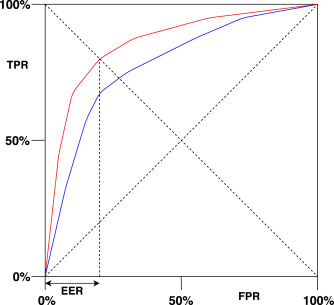
\includegraphics[width=.38\textwidth]{images/roc-curve}
    \caption{Ejemplo de curvas ROC y cálculo del EER. Se espera que el
      modelo con la curva roja tenga sea más potente, ya que su AUC es
      mayor. La intersección entre la curva ROC y la línea diagonal
      marca dónde el FPR y el TPR son iguales, punto que se define
      como el EER.}
    \label{fig:roc-curve}
  \end{figure}
\end{itemize}

\subsection{Métricas a nivel de fotograma y a nivel de píxel}
\label{sec:frame-and-pixel-levels}

Dado que la detección de anomalías en vídeo está muy relacionada con
la detección de objetos en imágenes, algunos criterios de evaluación
de anomalías son similares a los utilizados en la detección de objetos.
En particular, se suelen utilizar dos tipos de métricas, las métricas
a nivel de fotograma y las métricas a nivel de píxel.\\

Cuando se trabaja a nivel de fotograma, cada fotograma completo del
vídeo se marca como normal o anómalo, sin tener en cuenta la posición
que ocupa la anomalía en la escena. Cuando la evaluación se realiza a
nivel de píxel, por el contrario, la anomalía se marca con una máscara
sobre el fotograma, que indica la posición exacta donde se produce la
anomalía. En este caso, la salida de los algoritmos debe ser una
máscara comparable a la anotación (puede ser una matriz binaria con el
tamaño de la imagen, las coordenadas de un rectángulo que encierre la
anomalía, etc), y se considera que la anomalía se ha identificado
correctamente si la máscara predicha coincide con la anotación
original. El criterio usual para considerar esta asociación es lo
que se conoce como métrica \textit{Intersection over Union (IoU)}.
Dado un rectángulo de anotación GT y un rectángulo de predicción PB,
la IoU entre GT y PB se define como:

\[ IoU(GT, PB) = \frac{\vert GT \cap PB \vert}{\vert GT \cup PB \vert} \]

Una anomalía se considera detectada si la métrica anterior entre la
predicción y la anotación correspondiente es superior a un valor
definido de antemano, usualmente $IoU(GT,PB) \geq 0.5$. Una vez se ha
establecido la correspondencia entre las predicciones y las
anotaciones, se realizan los siguientes cálculos: las predicciones
correctamente asociadas a una anotación se consideran verdaderos
positivos, las predicciones que no tienen una anotación asociada se
consideran falsos positivos, y las anotaciones que no tienen una
predicción son falsos negativos. Adicionalmente, si las anotaciones
tienen una etiqueta de comportamiento normal o anómalo, aquellas
anotaciones con etiqueta de comportamiento normal que no han recibido
ninguna predicción son consideradas verdaderos negativos.

\section{Revisión de la literatura}

En esta sección se va a desarrollar una revisión bibliográfica de los
trabajos que resuelven el problema de la detección de anomalías
empleando redes neuronales profundas en algún paso de la solución.
Dividiremos la sección en función del tipo de anomalía que resuelvan,
y tras esa división, agruparemos los trabajos en función del tipo de
modelo empleado. En la sección \ref{sec:motion-appearance-revision} se
muestran los trabajos que afrontan el problema de la detección de
anomalías de movimiento y de apariencia. Se han combinado estos dos
subproblemas dado que usualmente se resuelven conjuntamente. En
particular, UCSD Pedestrians Dataset, el conjunto de datos más
utilizado para la detección de movimiento anómalo, marca estos dos
tipos de anomalía indistintamente en sus anotaciones, por lo que la
mayoría de trabajos resuelven ambos problemas simultáneamente. En la
sección \ref{sec:action-revision} se presentan los trabajos que
resuelven la detección de acciones anómalas, y en la sección
\ref{sec:position-revision} se expone el trabajo que se centra
en detectar posiciones anómalas.

\subsection{Detección de movimiento y apariencia anómala}
\label{sec:motion-appearance-revision}

En esta sección se revisan aquellos trabajos que utilizan modelos
basados en aprendizaje profundo (Deep Learning, DL por sus siglas en
inglés) para la detección de anomalías de movimiento y apariencia,
agrupando dichos trabajos en función del tipo de modelo que utilizan
para resolver la tarea.

\subsubsection{Extracción de características con DL y SVM monoclase}
\label{sec:oneclass-svm}

Una aproximación común a este problema consiste en la utilización de
modelos profundos para la extracción de características, y el uso de
estas características en una etapa posterior de entrenamiento de un
modelo de SVM monoclase. Las SVM monoclase \cite{scholkopf2000support}
son una clase particular de SVM cuyo objetivo es encontrar la frontera
de decisión más pequeña tal que los ejemplos normales con los que
se ha entrenado queden dentro de dicha frontera. De esta forma, al
clasificar nuevos ejemplos, aquellas características que quedan fuera
de la región normal aprendida son clasificadas como anomalías.\\

En \cite{xu2015learning} se propone un modelo basado en tres
\textit{Denoising AutoEncoders} (estructuras autocodificadoras para
eliminación de ruido) \cite{vincent2008extracting}, que aprenden a
reconstruir los fotogramas originales del vídeo (lo que extrae
características de apariencia), el flujo óptico de los fotogramas
\cite{horn1981determining} (lo que extrae características de
movimiento) y la concatenación de ambos (que aprende características
conjuntas). Una vez están entrenados los tres \textit{AutoEncoders},
se utiliza la representación latente de cada modelo (es la capa en la
que se obtiene la representación más reducida de cada fotograma) para
entrenar tres SVMs monoclase. Finalmente, un modelo combinado por voto
de las tres máquinas de soporte vectorial decide la clasificación
final. De forma similar, Gutoski et al. \cite{gutoski2017detection}
Utiliza un \textit{AutoEncoder} convolucional para reconstruir el
fotograma de entrada, su flujo óptico y los ejes detectados con el
detector de ejes de Canny de la imagen \cite{canny1986computational}.
En una segunda etapa, se calculan los errores de reconstrucción de
cada canal por separado, y se entrena una SVM sobre dichos 3
valores. Se realizan dos experimentos en este artículo. En el primero,
se marcan regiones anómalas, lo que permite una evaluación a nivel de
píxel. En el segundo, se marcan fotogramas enteros, utilizando el
valor máximo encontrado en la imagen.\\

Los autores de \cite{yang2019deep} proponen un modelo combinado
utilizando dos \textit{Autoencoders} de eliminación de ruido. Uno de
ellos trabaja con el vídeo original, mientras que el otro recibe el
primer plano de la escena, calculado utilizando el descriptor de
Kanade-Lucas-Tomasi \cite{lucas1981iterative}. Para ambas entradas, se
calcula el mapa de movimiento de la imagen y se introduce en el
modelo.  Una vez se han extraído las características en el espacio
latente, se lleva a cabo una reducción de dimensionalidad con una red
de creencia profunda (DBN) \cite{hinton2006fast}, y la representación
reducida se introduce en la SVM para cada modelo. La puntuación de
anomalía para cada fotograma se calcula finalmente como una
combinación lineal de las salidas de ambos modelos. Se puede observar
un esquema de este modelo en la figura \ref{fig:sdae-psvm}.\\

\begin{figure}[hbtp]
  \centering
  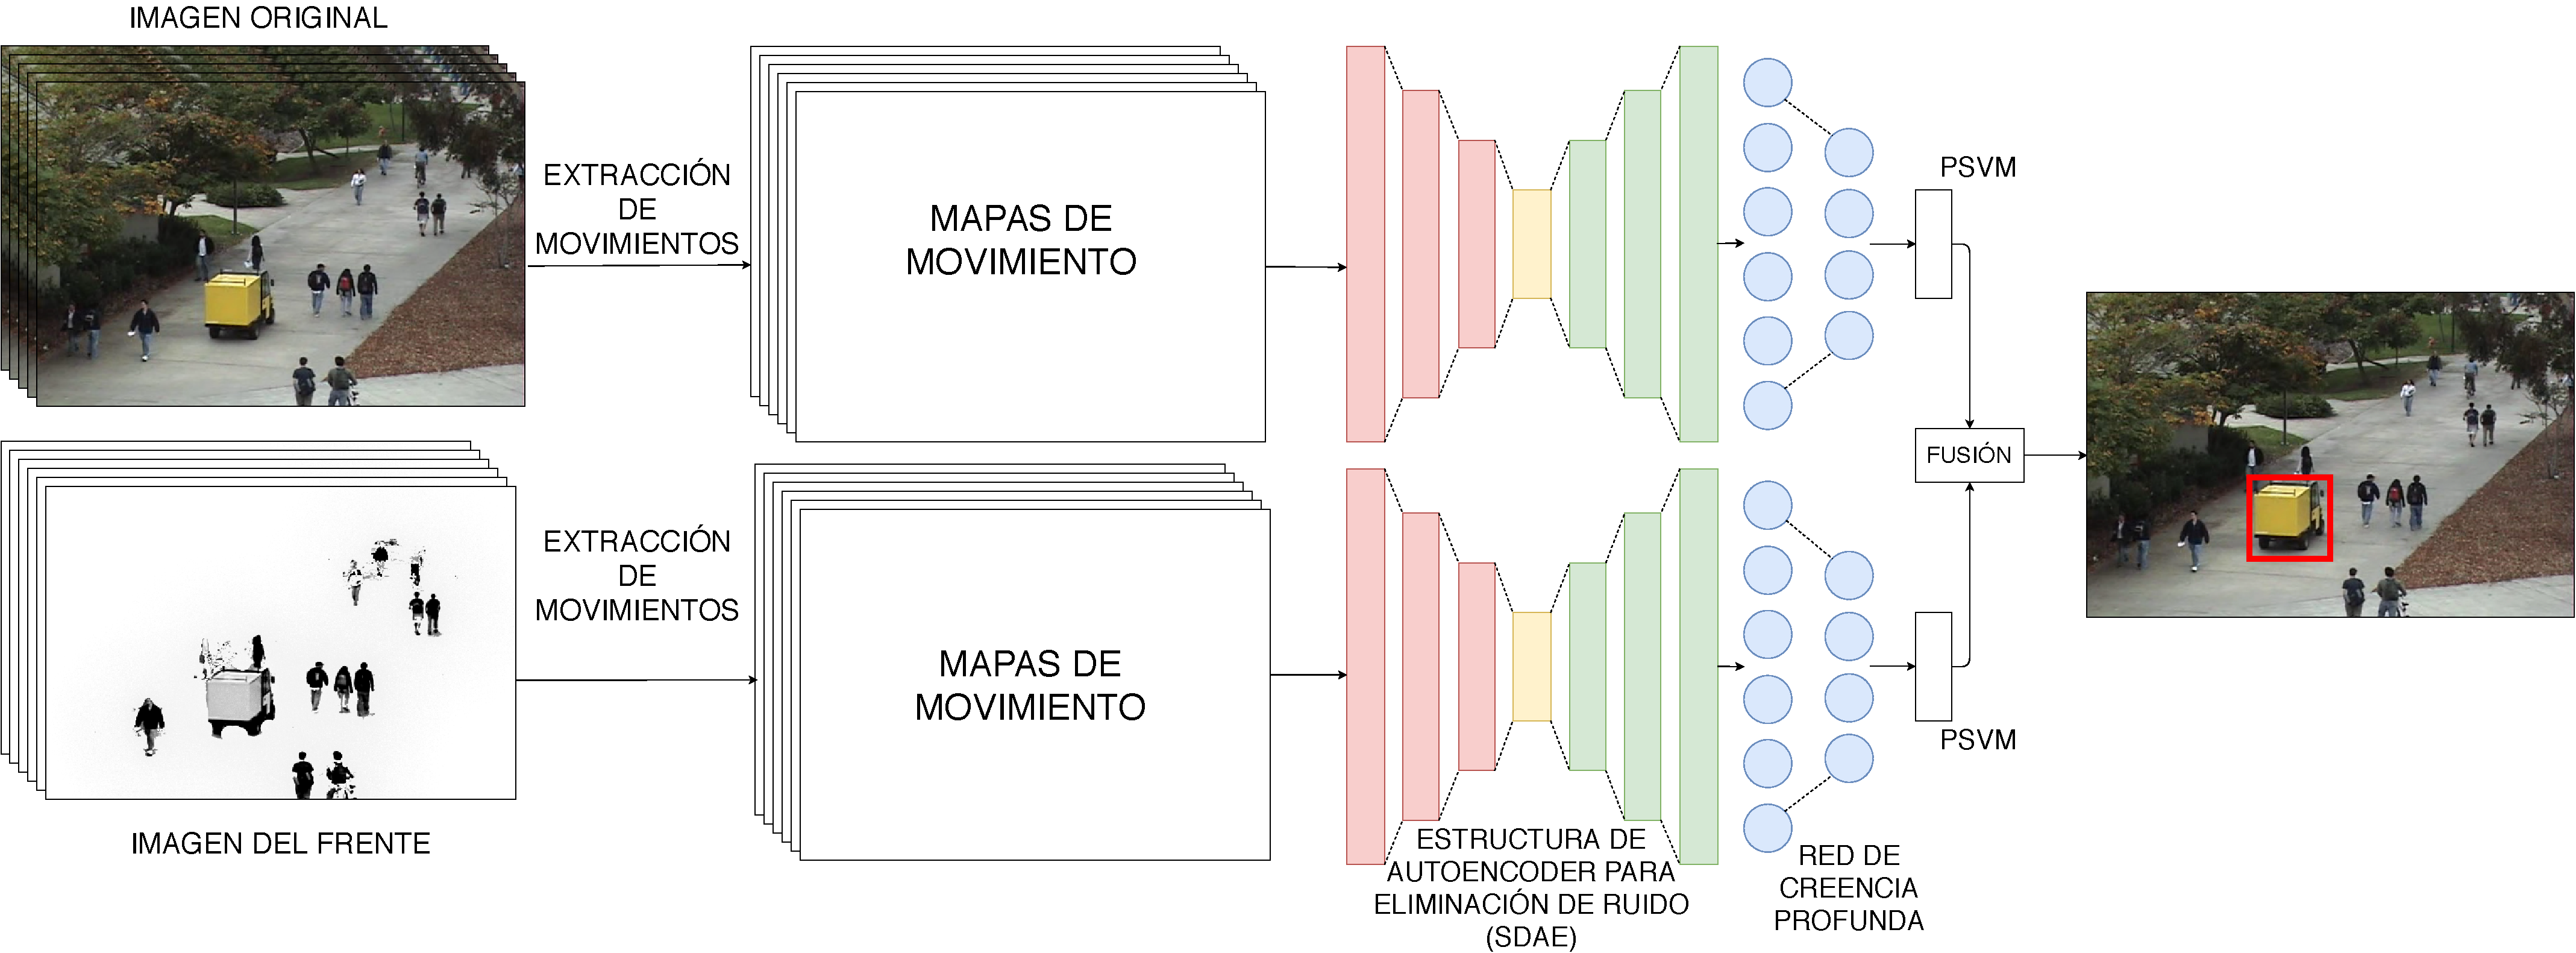
\includegraphics[width=.9\textwidth]{images/sdae_psvm.pdf}
  \caption{Ejemplo de SVM monoclase para detección de anomalías. Dos
    estructuras autocodificadoras reciben los mapas de movimiento de
    las imágenes originales y sus correspondientes secuencias sin
    fondo, y tratan de reconstruir la informcación original. Se reduce
    la dimensionalidad de la representación latente con una red de
    creencia profunda y se utiliza una SVM monoclase para aprender el
    patrón usual.}
  \label{fig:sdae-psvm}
\end{figure}

Fang et al. \cite{fang2016abnormal} utilizan dos características
clásicas, los mapas de atención (saliency maps) \cite{fang2011bottom}
y los histogramas de flujo de movimiento multiescala para entrenar una
red neuronal profunda denominada PCANet \cite{chan2015pcanet}.  Dicha
red neuronal trata de aprender a hacer un análisis de componentes
principales en cascada, lo que produce una reducción de
dimensionalidad de la entrada. Tras la reducción de dimensionalidad,
una SVM monoclase aprende el patrón normal de características. En
\cite{smeureanu2017deep}, se utiliza un modelo VGG-f
\cite{chatfield2014return} preentrenado como extractor de
características, y se entrena una SVM sobre las características
visuales extraídas. El uso de una red relativamente poco profunda hace
que el modelo consiga funcionar a unos 20 fotogramas por segundo, lo
que permite su uso en aplicaciones en tiempo real, consiguiendo unos
resultados relativamente similares a los obtenidos con redes más
profundas. De forma similar, Sun et al. \cite{sun2019abnormal} diseñan
una capa especial de SVM monoclase, la cual colocan al final de una
red neuronal convolucional, de forma que pueden entrenar el modelo
completo de una sola vez.\\

En \cite{singh2020crowd} se propone un modelo de unión de tres modelos
simples. Se entrenan tres modelos basados en redes convolucionales
(concretamente, un modelo VGG, un modelo AlexNet y un modelo
GoogLeNet), y sus salidas se concatenan para formar vectores de
características. Tras esto, los vectores de características se utilizan
para entrenar distintos modelos de SVM monoclase, cuya salida se combina
para establecer la clasificación final.\\

Huang et al. \cite{huang2018learning} proponen también un modelo de
combinación de características, extraídas utilizando máquinas de
Boltzmann convolucionales \cite{lee2009convolutional}. Se entrenan
tres modelos distintos, utilizando como entrada regiones de la imagen
original, regiones extraídas de la transformada por convolución
gaussiana, y regiones extraídas del flujo óptico del vídeo. Las
características extraídas sobre estas tres entradas se concatenan y se
introducen en una SVM monoclase que aprende los patrones de movimiento
comunes.\\

Un ejemplo interesante puede encontrarse en
\cite{hinami2017joint}. Los autores proponen un modelo entrenado en
dos fases. En una primera etapa, se entrena una versión modificada del
detector Fast R-CNN \cite{girshick2015fast} para que realice
aprendizaje multitarea. Dicho entrenamiento se lleva a cabo de forma
supervisada sobre conjuntos de gran tamaño, de forma que el modelo es
capaz de extraer información semántica de los objetos que hay en la
escena. En una segunda etapa, con el extractor semántico genérico ya
entrenado, un detector de anomalías aprende el patrón normal
específico para cada dataset en el que se quiera aplicar el método, y
devuelve una puntuación de anomalía en tiempo de inferencia. En el
artículo se ofrecen resultados con distintos detectores de anomalías,
obteniéndose los mejores resultados con las SVMs monoclase. La ventaja
de esta aproximación es su carácter genérico, ya que el extractor de
características puede usarse en muchos contextos distintos. Esto hace
que este método pueda utilizarse también para la detección de acciones
anómalas. No obstante, se ha incluido en esta sección porque los
autores muestran sus resultados utilizando el UCSD Peds1.

\subsubsection{Extracción de características con DL y modelos gaussianos}

Otro enfoque muy utilizado consiste en aprender una distribución de
probabilidad sobre las características, usualmente utilizando
distribuciones gaussianas, y considerando como anomalías aquellos
ejemplos cuya probabilidad es baja respecto a la distribución
aprendida. En este caso, de nuevo se extraen las características
utilizando modelos de aprendizaje profundo.\\

En \cite{sabokrou2015real}, se aprenden dos descriptores distintos.
Por un lado, el vídeo se divide en parches 3D no solapados (regiones
de la escena en varios fotogramas consecutivos), y se calculan
descriptores globales y locales. Los descriptores locales se calculan
a partir de una medida de similaridad entre el parche en cuestión y
sus vecinos, mientras que el descriptor global es una representación
latente aprendida con un modelo de \textit{AutoEncoder}. En ambos
casos, se aprende un modelo Gaussiano sobre los descriptores
obtenidos, y en tiempo de inferencia se considera que un ejemplo es
anómalo si ambos modelos marcan como anomalía a dicho parche. Los
mismos autores ofrecen un refinamiento del modelo en
\cite{sabokrou2017fast}. En este caso, se utiliza el descriptor local
como un primer filtro rápido para los parches sencillos. Cuando hay
que clasificar un parche nuevo, si el modelo que ha aprendido sobre
los descriptores locales devuelve como respuesta que el parche es
normal, se termina la clasificación. Si se devuelve que el parche es
anómalo, se computa el descriptor global y se clasifica con su modelo,
que establece la clasificación final. De esta forma, se consigue un
modelo con la potencia del descriptor global, que obtiene mejores
resultados, pero con una reducción importante de cómputo, ya que el
descriptor local es más sencillo de calcular.\\

Los mismos autores proponen también un modelo basado en cascada en
\cite{sabokrou2017deep}. En este caso, el primer discriminante
funciona con el error de reconstrucción obtenido por un
\textit{AutoEncoder} poco profundo, que elimina rápidamente los
parches simples (especialmente los parches compuestos por fondo,
ya que el error de reconstrucción en este caso es muy bajo).
A continuación, una red convolucional en tres dimensiones se entrena
para extraer características de los parches no descartados. Con las
características extraídas por la red, se aprende el modelo Gaussiano,
utilizando la distancia de Mahalanobis entre las características
de los nuevos parches y los parches de entrenamiento.\\

Feng et al. \cite{feng2017learning} proponen un método basado en
gradientes en tres dimensiones. Para cada vídeo a clasificar, se
calculan los gradientes en vertical, horizontal, y dimensión temporal,
y se entrena una red PCANet \cite{chan2015pcanet} sobre dichos
descriptores. Sobre las características extraídas por la red, se
entrena un modelo de mezcla de gaussianas profundo
\cite{viroli2019deep}. Dicho modelo es una adaptación de los modelos
de mezcla de gaussianas de forma que pueden entrenarse como una red
neuronal, utilizando optimización basada en el gradiente descendente.
En tiempo de inferencia, si la salida del modelo gaussiano profundo
está por debajo de un umbral, significa que la probabilidad de que
la entrada ocurra es baja, y por tanto se marca el fotograma como
anomalía.

\subsubsection{Modelos basados en técnicas de reconstrucción}

La idea que subyace en el funcionamiento de estos modelos consiste en
entrenar un modelo capaz de reconstruir la imagen de entrada original
a partir de su representación latente. Tras entrenar los modelos
utilizando solamente imágenes normales, el resultado de aplicar estos
modelos sobre imágenes anómalas produce reconstrucciones irregulares.
Por tanto, calculando el error cometido en la reconstrucción se obtiene
una medida de la irregularidad del fotograma de entrada.\\

Un ejemplo de esta técnica se puede encontrar en Ramchandran et al.
\cite{ramchandran2019unsupervised}. Los autores entrenan un
\textit{AutoEncoder} convolucional (CAE) con estructura recurrente
basada en un modelo LSTM. Dicho modelo es un CAE con una configuración
recurrente, de forma que puede trabajar directamente con secuencias de
vídeo, y no exclusivamente con imágenes. En particular, el modelo
LSTM-CAE (como lo denominan los autores), aprende a reconstruir
fragmentos originales del vídeo a partir de las aristas detectadas en
sus fotogramas utilizando el detector de Canny. Cuando un segmento
anormal de vídeo es reconstruido en tiempo de inferencia, el error
de reconstrucción cometido crece considerablemente, lo que permite
definir un umbral a partir del cual se considera que un fragmento
es anómalo.\\

Otro ejemplo de error de reconstrucción se encuentra en
\cite{ravanbakhsh2018plug}. En este trabajo, se construye una CNN con
estructura temporal y salida binaria, que traduce un vídeo de entrada
en un conjunto de características binarias. Utilizando dichas
características, se aprende un diccionario de códigos binarios, y cada
fragmento de vídeo se representa como un histograma de dichos códigos.
En tiempo de inferencia, la irregularidad de dicho histograma, medida
como la cantidad de información que se pierde al representar el vídeo
utilizando el diccionario, contiene información sobre el grado de
anomalía del vídeo. Además, para calcular la región anómala con mayor
precisión, se utiliza un sistema basado en el flujo óptico.

\subsubsection{Modelos completos basados en aprendizaje profundo}

Algunos autores han entrenado redes neuronales profundas cuya salida
es directamente una puntuación de anomalía, en lugar de utilizar los
modelos profundos como extractores de características sobre los que
luego se entrena un modelo clásico. La principal ventaja de este
enfoque es que los modelos pueden ser entrenados en un solo paso,
sin necesidad de aplicar distintas etapas de entrenamiento.\\

Zhou et al. \cite{zhou2016spatial} definen un modelo espacio-temporal
cuya salida es la probabilidad de que un determinado fragmento de
vídeo contenga una anomalía. En el algoritmo, cada vídeo se divide en
pequeños fragmentos, y se calcula el flujo óptico de los mismos. Si el
parche tiene un objeto en movimiento, lo cual se mide en función de la
magnitud del flujo, se considera que el fragmento es relevante y se
procesa por la red neuronal. Si no se detecta movimiento con el flujo
óptico, el fragmento se marca directamente como normal, para evitar
procesamiento innecesario y reducir el tiempo de cómputo. De nuevo,
este modelo se emplea también para la detección de acciones anómalas,
no sólo de movimiento, pero al estar la mayoría del trabajo centrado
en las anomalías de movimiento hemos decidido incluirlo en esta
sección.\\

En \cite{ravanbakhsh2019training} se entrenan dos redes generativas
adversarias (GANs \cite{goodfellow2014generative}). En el primero de
los modelos, el generador tiene que calcular el flujo óptico a partir
de las imágenes originales, mientras que en el segundo se tiene que
realizar la tarea inversa, es decir, calcular las imágenes originales
a partir del flujo óptico. En ambos casos, las GANs se entrenan
exclusivamente sobre fotogramas normales. En tiempo de inferencia,
sólo se utilizan los discriminantes, y dado que no se han entrenado
sobre fotogramas anómalos, el modelo tiende a marcar los mismos como
fotogramas falsos. La puntuación de anomalía se consigue finalmente
sumando los valores de ambas redes.

\subsubsection{Otros enfoques}

Algunos de los modelos estudiados siguen enfoques completamente
distintos a los comentados anteriormente. En \cite{kumar2017d}, se
propone un modelo en cascada. En una primera etapa, una CNN poco
profunda descarta los parches de vídeo normales (usualmente los
compuestos por fondo). Si dicha CNN no es capaz de marcar el fragmento
como normal, se procesa el fragmento con una CNN más profunda. Las
características visuales extraídas por la CNN se utilizan para
estudiar el modelo de movimiento de los sujetos de la imagen
utilizando un filtro de Kalman flexible. Dicho modelo es una
modificación del filtro de Kalman clásico, en el que se mide cuánto se
desvía el sujeto del modelo de movimiento normal. Dicha desviación
se utiliza como medida de la anomalía.\\

La propuesta de Hu et al. tiene un enfoque interesante. En su trabajo
proponen un nuevo modelo profundo, llamado D-IncSFA, cuyo objetivo es
llevar a cabo una reducción de dimensionalidad utilizando una técnica
llamada análisis de características lentas (\textit{Slow Feature
  Analysis}, SFA \cite{wiskott2002slow}). Dicha técnica de reducción
de dimensionalidad trabaja sobre series temporales, y trata de aislar
aquellas características con cambio más lento que definen una señal.
Dado que el cálculo de SFA es computacionalmente muy costoso, la red
aprende a calcular una aproximación de dicha a transformada. Tras ser
entrenada sobre vídeos normales, la puntuación de anomalía se define
como el cuadrado de las derivadas de la señal de salida. Dado que
el modelo SFA es entrenado sólo sobre vídeos normales, al aplicarlo
sobre vídeos anómalos la salida crece significativamente, lo que
indica una anomalía. Se proponen dos soluciones distintas a partir
de este modelo. Por un lado, para la detección de anomalías a nivel
de fotograma, se toma la salida de la última capa y se calcula el
máximo. Para la detección a nivel de píxel, se combina la salida
de cinco capas distintas de la red, utilizándolas como mapas de
características a distintas escalas.

\subsection{Detección de acciones anómalas}
\label{sec:action-revision}

En esta sección se revisan los modelos especializados en la detección
de acciones anómalas. Estos trabajos no se han dividido por tipos de
modelos ya que el número de trabajos dentro de este apartado es
significativamente menor que en el caso anterior.\\

Siguiendo sus trabajos anterior en detección de movimiento anómalos,
Sabokrou et al. \cite{sabokrou2018deep} proponen un clasificador en
cascada.  Utilizando una red completamente convolucional basada en
AlexNet y preentrenada, se extraen parches de características
multiescala para cada fotograma. A partir de esta información, se
entrenan dos clasificadores gaussianos. Un primer clasificador utiliza
exclusivamente la información de las primeras $k$ capas más
superficiales de la red, y se aprende un clasificador simple.  Si la
predicción de dicho clasificador es segura (dos valores marcan si el
comportamiento es normal o anormal con certeza), la clasificación se
considera terminada. Si la predicción no es clara (se obtiene un valor
en el intervalo central), se calculan características con capas más
profundas para refinar la decisión, a costa de un coste computacional
mayor.\\

Los errores de reconstrucción también se han utilizado para la
detección de acciones anómalas. Un ejemplo de este tipo de modelos se
encuentra en \cite{wang2019abnormal}. En este trabajo se entrenan dos
\textit{AutoEncoders} para reducción de ruido capaces de extraer
información visual y de movimiento de las trayectorias detectadas
en el vídeo. Tras la extracción de características por parte de los
\textit{AutoEncoders}, se calcula una representación por bolsa de
palabras, y el error de reconstrucción de las características
originales a partir de su representación en la bolsa de palabras se
considera una puntuación de anomalía.\\

En \cite{sultani2018real} se propone un modelo completamente basado en
aprendizaje profundo para dar solución al problema. En su trabajo, la
detección de anomalías se describe como un aprendizaje débilmente
supervisado, desde el punto de vista del aprendizaje multiinstancia.
Dado que en su trabajo utilizan un conjunto de datos etiquetado a
nivel de vídeo, en lugar de a nivel de fotograma (esto es, los vídeos
etiquetados como anómalos no marcan en qué fragmento del vídeo se
sitúa la anomalía), el vídeo se divide en pequeños fragmentos que
forman una bolsa de ejemplos. Los vídeos en los que se sabe que existe
una anomalía forman bolsas positivas, y los vídeos normales forman
bolsas negativas. Sobre los fragmentos de las bolsas se utiliza un
extractor de características del tipo 3D CNN, y sobre dichas
características se entrena una red completamente conectada, con una
función de coste adaptada al aprendizaje multiinstancia. Nos
centraremos en este modelo en capítulos posteriores, ya que nos
servirá de base a la hora de diseñar nuestro modelo.\\

Los autores de \cite{tay2019robust} resuelven el problema de la
detección de acciones anómalas utilizando un enfoque híbrido entre
la detección de anomalías y la clasificación de eventos. Una red
convolucional se entrena para distinguir entre 6 tipos distintos
de eventos anómalos, dados un conjunto de fotogramas de una secuencia
de vídeo anómala. En el trabajo se llevan a cabo dos experimentos
distintos. En primer lugar, la salida de la red es una etiqueta
binaria, la cual indica si en el vídeo se encuentra presente o no
una anomalía. En el segundo experimento, la categoría concreta
del comportamiento anómalo, si está presente, se especifica también
como salida.\\

Las escenas de violencia han sido ampliamente estudiadas en el
contexto de la detección de acciones anómalas. Uno de los primeros
ejemplos del uso de aprendizaje profundo para la detección de
violencia se puede encontrar en \cite{kecceli2017violent}. En este
trabajo, se calculan cuatro mapas de características clásicos, todos
ellos derivados del flujo óptico de la imagen. Estos mapas de
características codifican información sobre orientación, magnitud y
velocidad de dicho flujo. Esta información se procesa con un modelo
AlexNet preentrenado que extrae características. A continuación, se
lleva a cabo una selección de características utilizando el algoritmo
Relief-F \cite{kononenko1997overcoming}. Con la representación
reducida, se prueban dos detectores de anomalías, una SVM monoclase y
un modelo basado en k-NN. Ese mismo año, Sudhakaran et
al. \cite{sudhakaran2017learning} proponen un modelo de entrenamiento
en una fase compuesto por una red completamente convolucional seguida
de una red recurrente LSTM para aprendizaje de los patrones de
movimiento. Finalmente, un conjunto de capas completamente conectadas
realizan la clasificación final. La particularidad de este modelo es
que afronta el problema desde el punto de vista del aprendizaje
supervisado, pero hemos decidido incluirlo aquí para dar una visión
más completa de la detección de violencia. En la figura
\ref{fig:cnn-lstm-violence} puede observarse un esquema del
funcionamiento de este modelo.\\

\begin{figure}[hbtp]
  \centering
  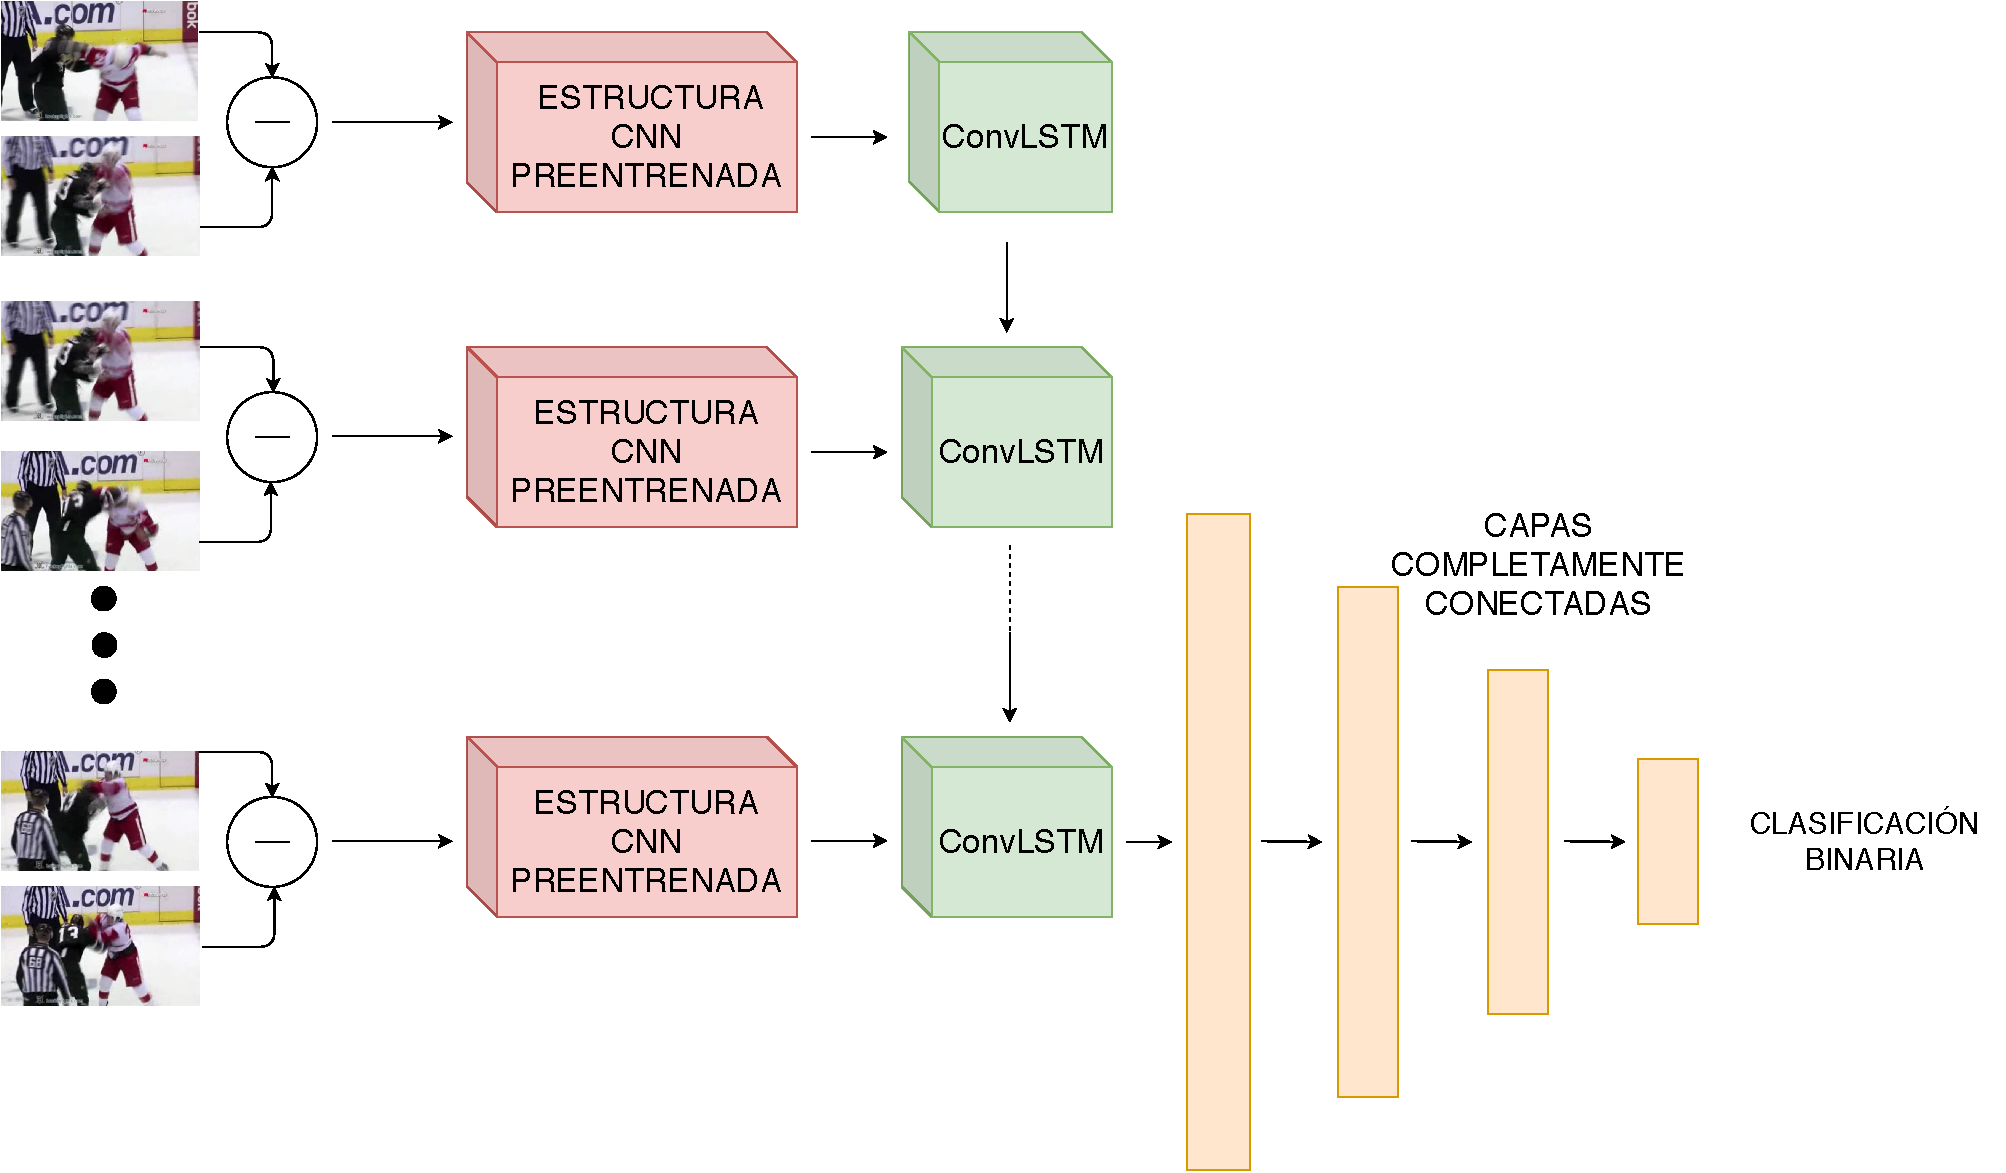
\includegraphics[width=.9\textwidth]{images/cnn_lstm_violence.pdf}
  \caption{Ejemplo de arquitectura para detección de violencia. El
    modelo de la imagen utiliza una arquitectura llamada
    CNN-LSTM. Consiste en una red convolucional cuya salida es utiliza
    por una LSTM convolucional que aprende patrones temporales. Tras
    la extracción de patrones temporales, un grupo de capas densas
    produce la clasificación final. Imagen adaptada de
    \cite{sudhakaran2017learning}.}
  \label{fig:cnn-lstm-violence}
\end{figure}

Una solución interesante se propone en el trabajo de Marsden et al.
\cite{marsden2017resnetcrowd}. Dicho modelo es una red CNN multitarea
que resuelve conjuntamente el problema de la detección de violencia,
el conteo de individuos, y la estimación de densidad en multitudes.
Las salidas de dicha red son una etiqueta binaria indicando la
presencia o no de violencia en la imagen, una neurona de regresión que
devuelve el número de individuos, y un mapa de calor que indica la
densidad de personas. Además, en este trabajo se propone un conjunto
de 100 imágenes completamente anotadas que se han usado para el
entrenamiento del modelo. El principal inconveniente de este método es
que funciona exclusivamente con imágenes, y no está preparado para su
uso con secuencias de vídeo.\\

En \cite{song2019novel} se propone un modelo basado en redes
convolucionales 3D. Según los autores, la principal contribución de su
trabajo es el método de selección aleatorio de fotogramas. Los
fotogramas relevantes del vídeo se seleccionan utilizando un modelo
clásico de agrupamiento. Dados dos fotogramas relevantes consecutivos,
se eligen 16 fotogramas aleatorios entre ellos, y dicha información se
introduce en la red convolucional para extraer características
espacio-temporales. Estas características se introducen después en un
detector de anomalías, el cual no se especifica en el texto del
artículo. En \cite{fenil2019real}, se propone un modelo LSTM
bidireccional, modificado para ser utilizado en un entorno \textit{Big
  Data}. Los vídeos son procesados dentro del ecosistema Spark,y
una representación basada en el histograma de gradientes se calcula
para cada fotograma. Esta representación se introduce después en el
modelo recurrente, el cual aprende los patrones temporales de los
eventos violentos. De nuevo, se resuelve el problema desde el punto
de vista del aprendizaje supervisado.\\

Finalmente, en \cite{sumon2019violent} se realiza un estudio
comparativo entre distintos modelos basados en aprendizaje
profundo. Los autores muestran resultados utilizando modelos basados
en redes convolucionales y recurrentes, entrenadas con distintas
políticas, y dando una comparación numérica entre ellos. El conjunto
de datos utilizando está compuesto por varios vídeos extraídos de
YouTube, donde se presenta una multitud bastante densa con diversos
episodios de violencia. En este trabajo se concluye que los modelos
preentrenados son los que mejores resultados arrojan, debido al
reducido tamaño del conjunto de datos. Los modelos entrenados desde
cero suelen dar resultados peores, a pesar de ser más complejos,
por la cantidad de datos escasa de la que se dispone.

\subsection{Detección de posiciones anómalas}
\label{sec:position-revision}

Como hemos dicho anteriormente, este es el tipo de anomalía más
sencillo de detectar. Una anomalía producida por posición se da cuando
un sujeto no identificado entra en una zona restringida. Normalmente,
el flujo de funcionamiento de estos modelos consiste simplemente en una
detección de peatones, seguida de una etapa de solapamiento entre los
rectángulos detectados y las regiones del fondo restringidas.\\

Este flujo es utilizado en el trabajo de Cheng el al
\cite{cheng2017abnormal}. En este trabajo, se considera anomalía la
incursión en un área restringida dentro de un puerto. Los vídeos están
recogidos por una cámara aérea, y el modelo está compuesto por un
detector simple (SSD \cite{liu2016ssd}) refinado para la detección
exclusiva de peatones y una zona ilegal definida en el fondo de la
imagen. El sistema lanza una alarma cuando un trabajador del puerto
penetra en la zona ilegal.

\end{document}

%%% Local Variables:
%%% mode: latex
%%% TeX-master: "../main"
%%% End:
